\documentclass{standalone}
\usepackage{tikz}
\begin{document}
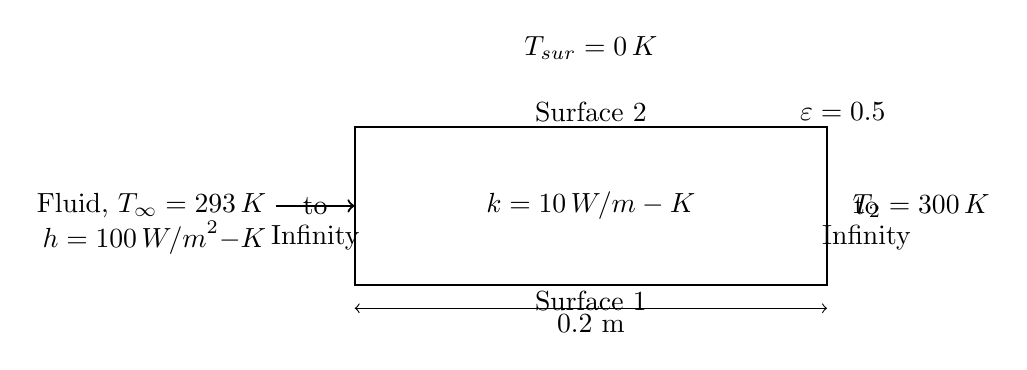
\begin{tikzpicture}
    % Draw the rectangle representing the block
    \draw[thick] (0, 0) rectangle (6, 2);

    % Draw labels for surfaces and sides
    \node at (-0.5, 1) {to};
    \node at (-0.5, 0.6) {Infinity};
    \node at (6.5, 1) {to};
    \node at (6.5, 0.6) {Infinity};
    \node at (3, 2.2) {Surface 2};
    \node at (3, -0.2) {Surface 1};

    % Draw and label heat transfer arrows
    \draw[->, thick] (-1, 1) -- (0, 1);
    \node[anchor=east] at (-1, 1) {Fluid, $T_{\infty} = 293\,\text{K}$};
    \node[anchor=east] at (-1, 0.6) {$h = 100\,\text{W/m}^2\text{-K}$};

    % Thermal conductivity and thickness
    \node at (3, 1) {$k = 10\,\text{W/m-K}$};
    \draw[<->] (0, -0.3) -- (6, -0.3);
    \node at (3, -0.5) {0.2 m};

    % Temperature on the right side
    \node[anchor=west] at (6.2, 1) {$T_2 = 300\,\text{K}$};

    % Surrounding temperature
    \node at (3, 3) {$T_{\text{sur}} = 0\,\text{K}$};

    % Emissivity label
    \node at (6.2, 2.2) {$\varepsilon = 0.5$};
\end{tikzpicture}
\end{document}
